\chapter{User Interface Design}
\section{Mockups}
The registered end users use a mobile interface, to use the services provided by the eMall system. It is an application that must be downloaded onto a mobile phone to be used. The mockpus of the interfaces are shown below.
\begin{table}[H]
\centering
\begin{tabu}to \textwidth {X[c]X[c]}
  
\includegraphics[width=30mm]{images/home.png}\captionof{figure}{Home page}\label{fig:homePageeMSP} &
  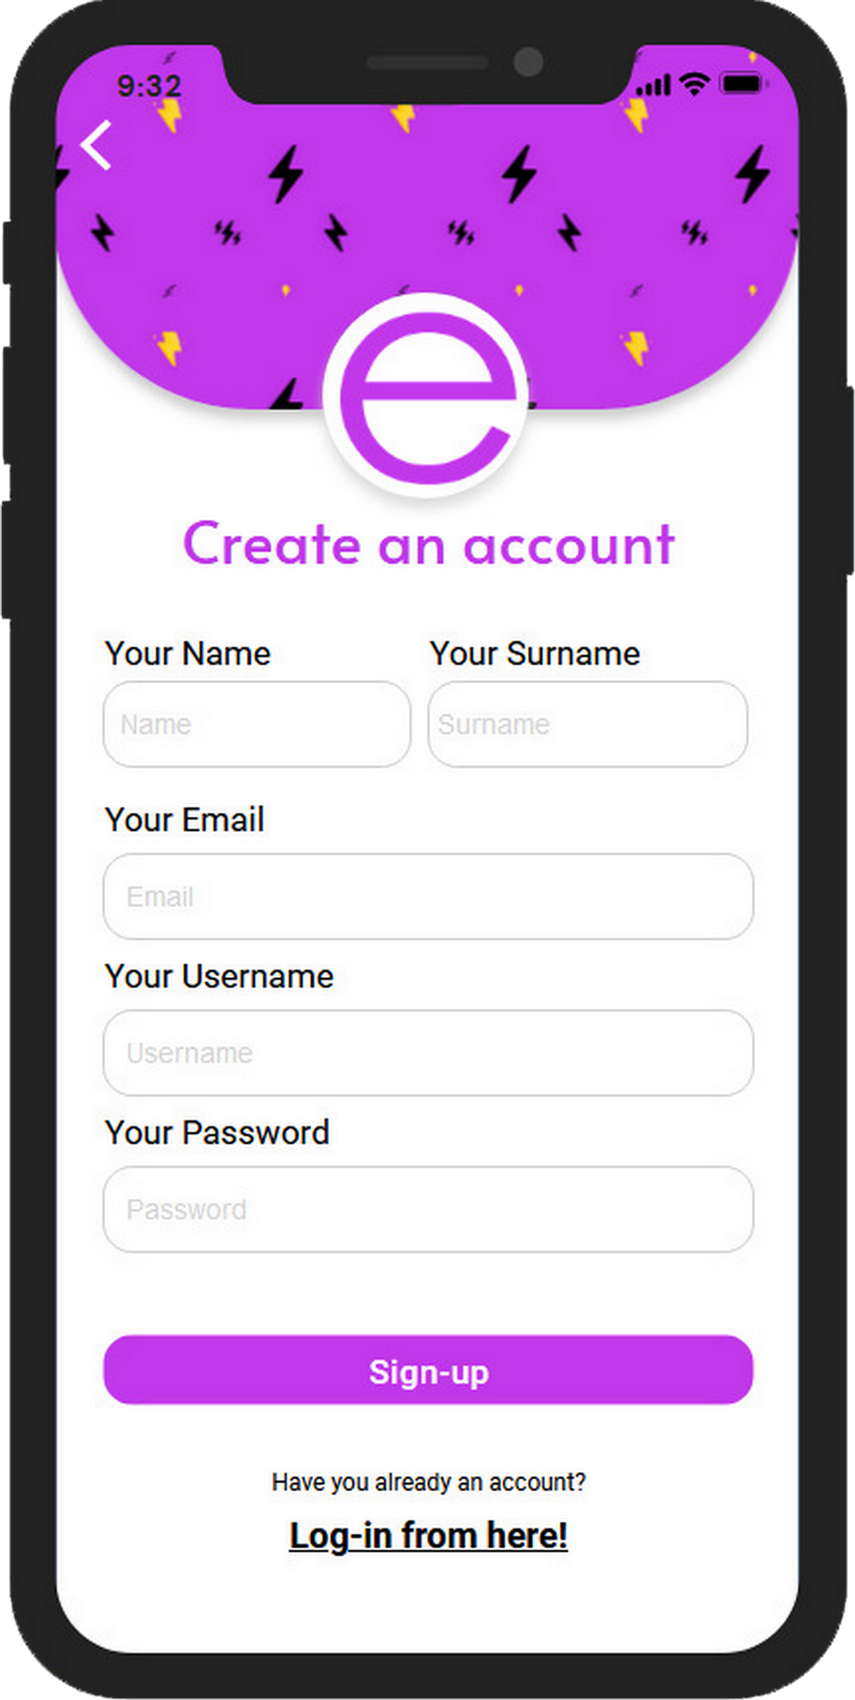
\includegraphics[width=30mm]{images/signup.png}\captionof{figure}{Sign up}\label{fig:signUpPage} \\
  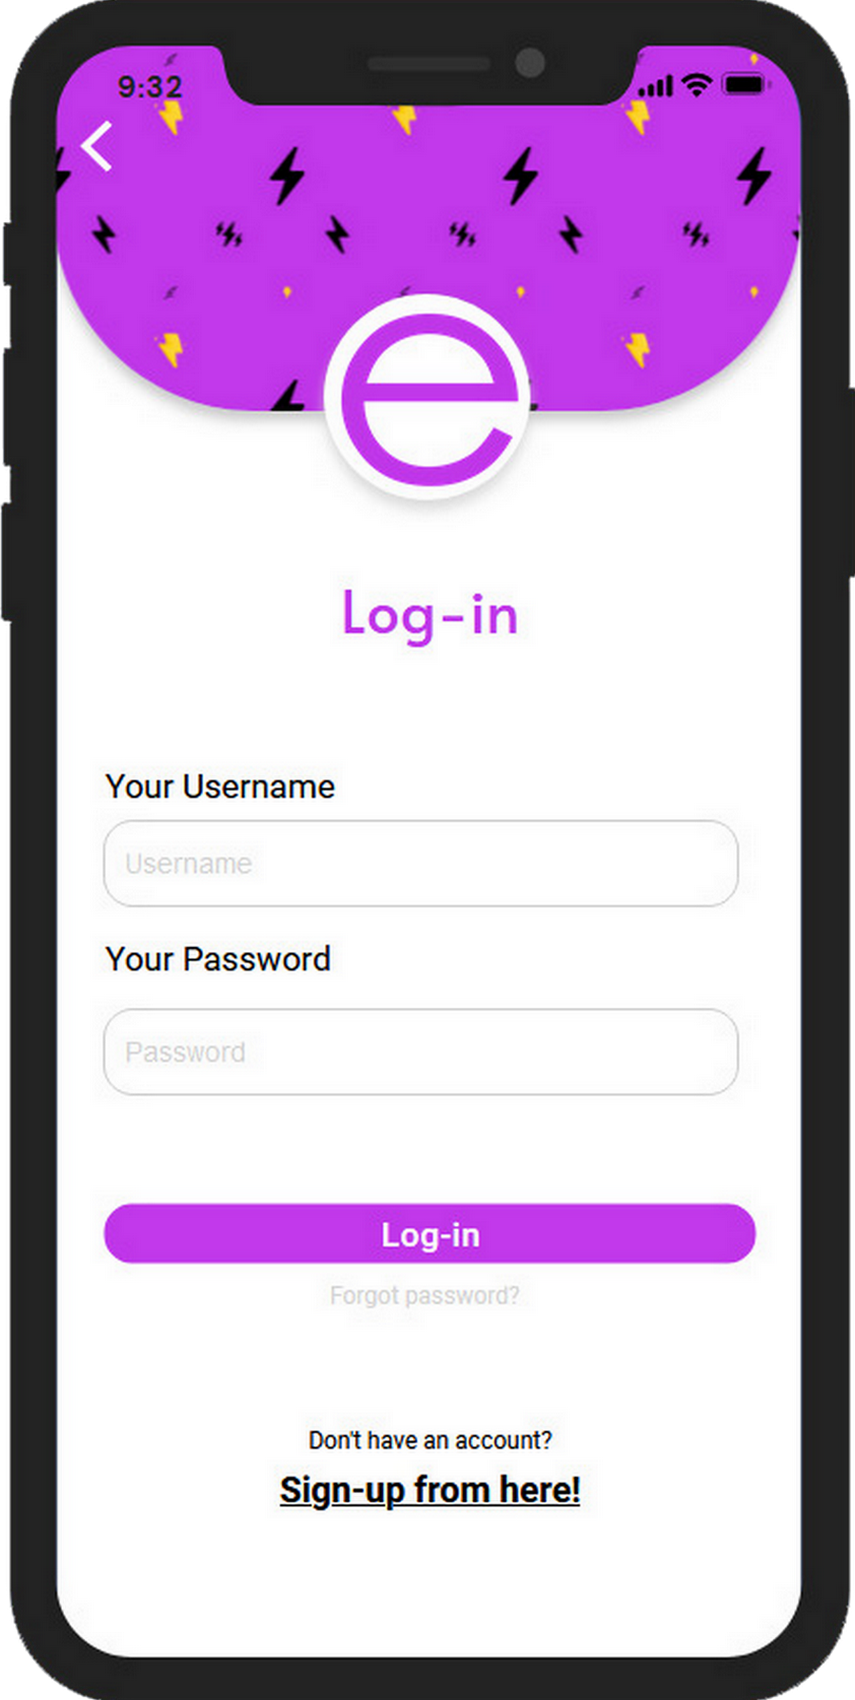
\includegraphics[width=30mm]{images/login.png}\captionof{figure}{Log-in}\label{fig:logInPage} &
  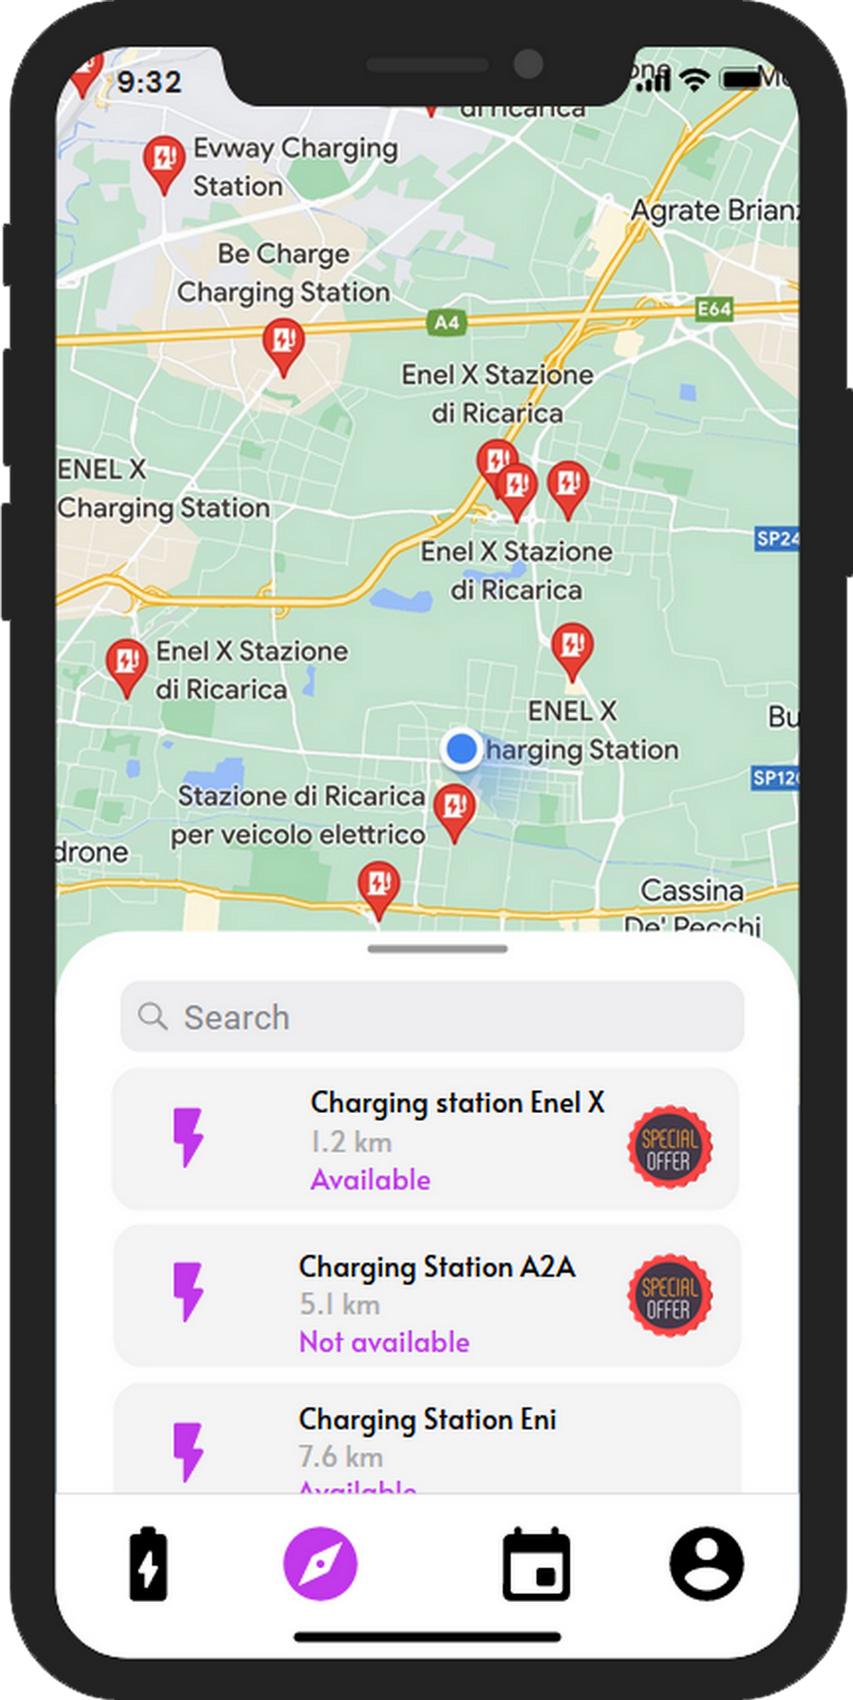
\includegraphics[width=30mm]{images/explore1.png}\captionof{figure}{Charging stations map}\label{fig:chargingStationMap} \\
\end{tabu}
\end{table}
\begin{table}[H]
\centering
\begin{tabu}to \textwidth {X[c]X[c]}
  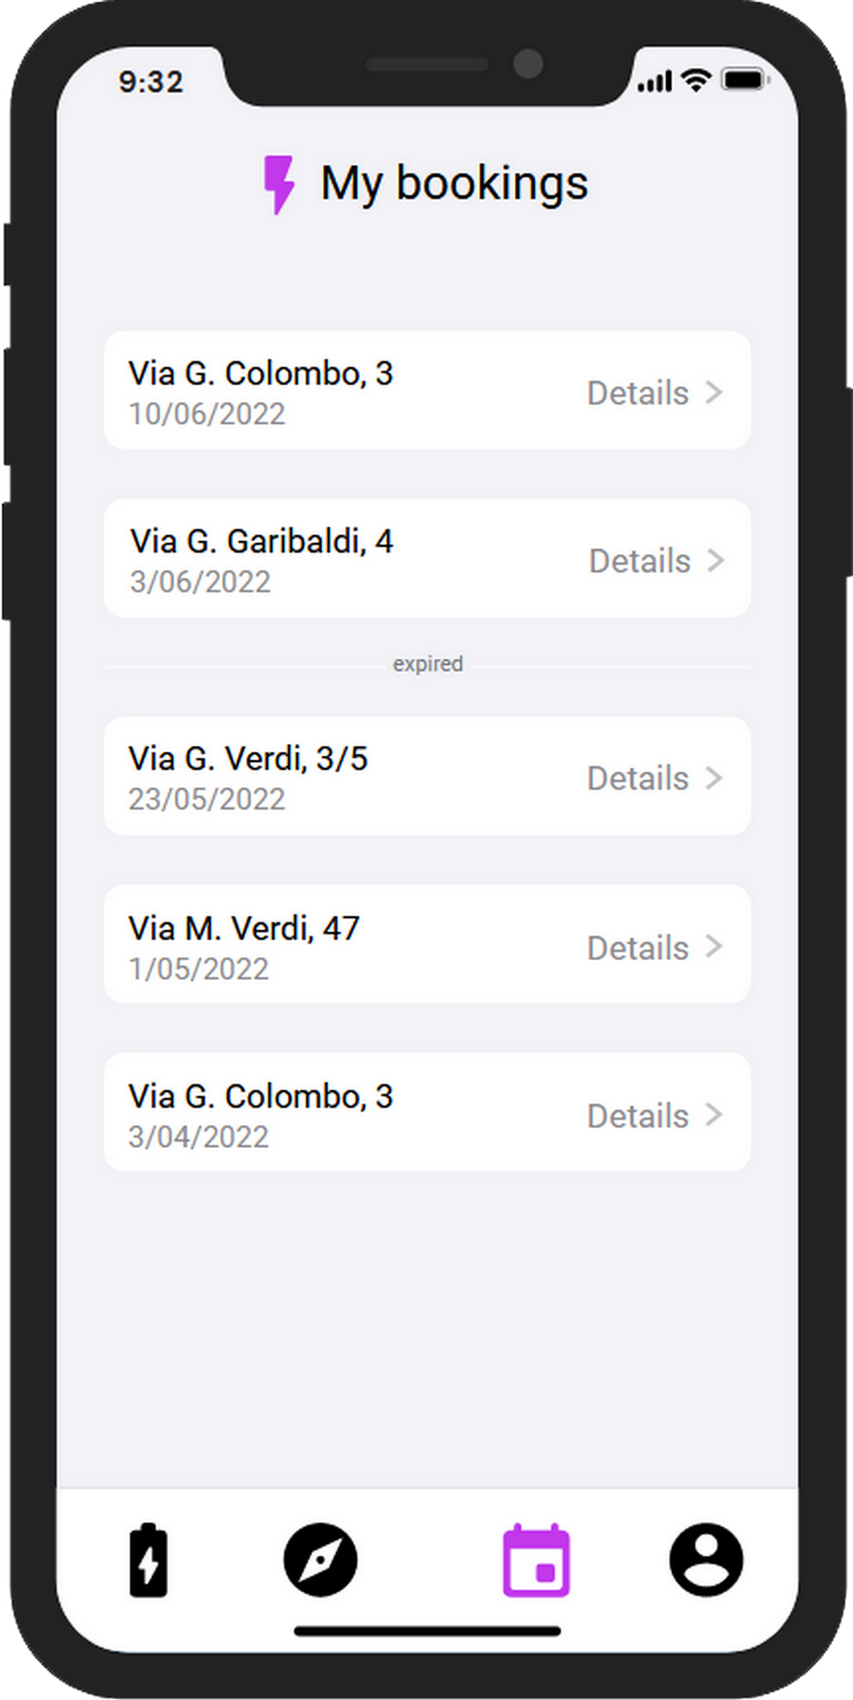
\includegraphics[width=30mm]{images/bookings.png}\captionof{figure}{My bookings}\label{fig:bookingPage} &
  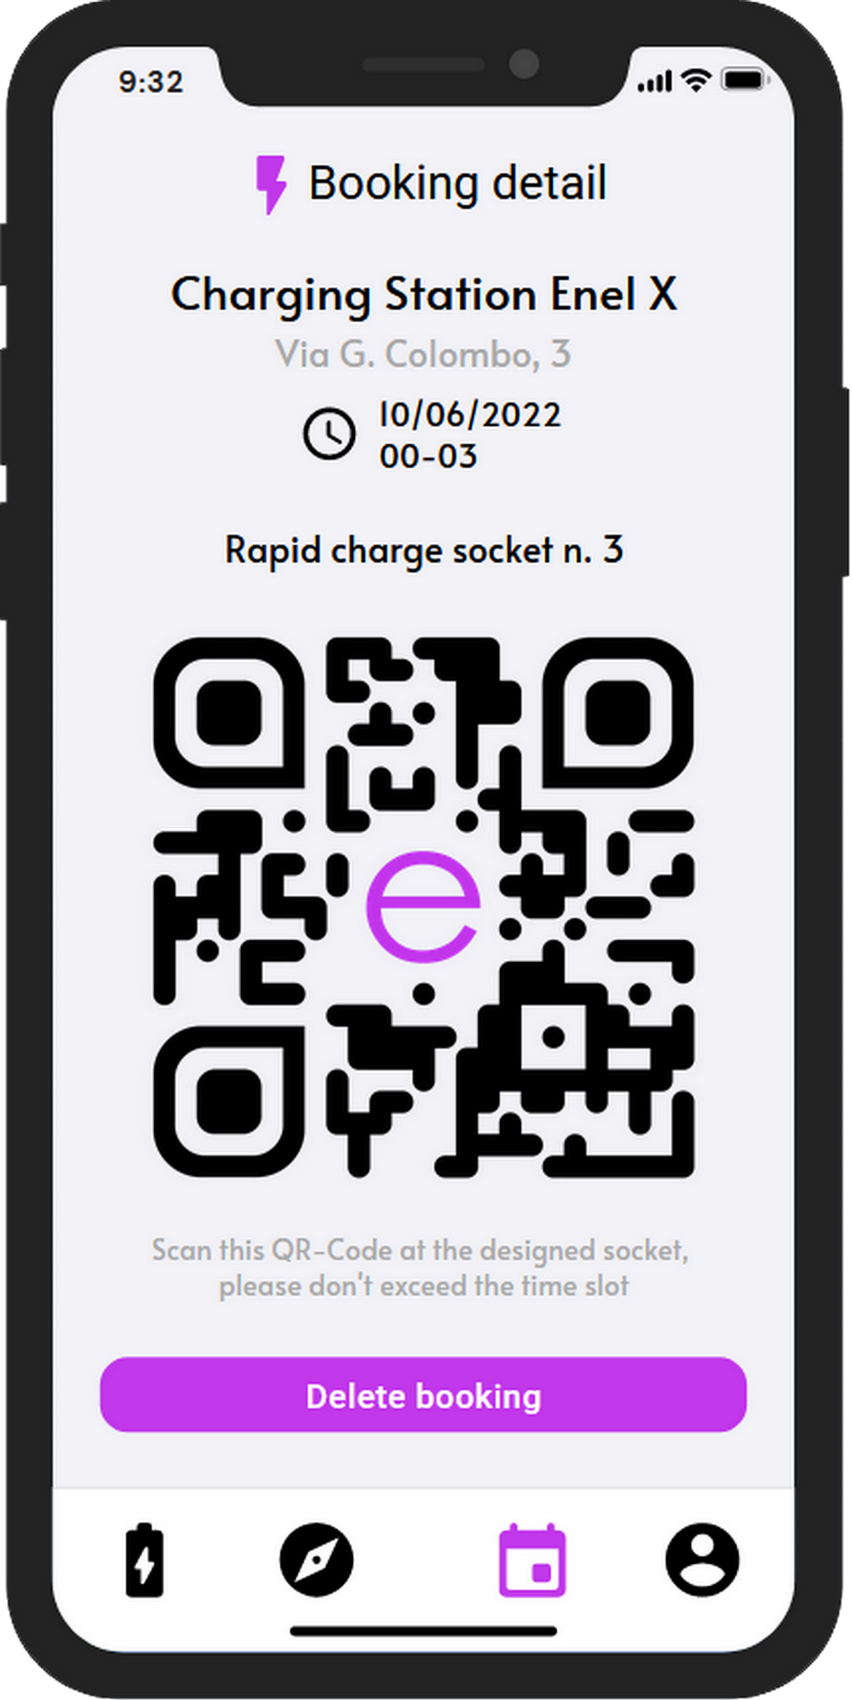
\includegraphics[width=30mm]{images/bookingdetail.png}\captionof{figure}{Bookings detail}\label{fig:qrCodePage} \\
  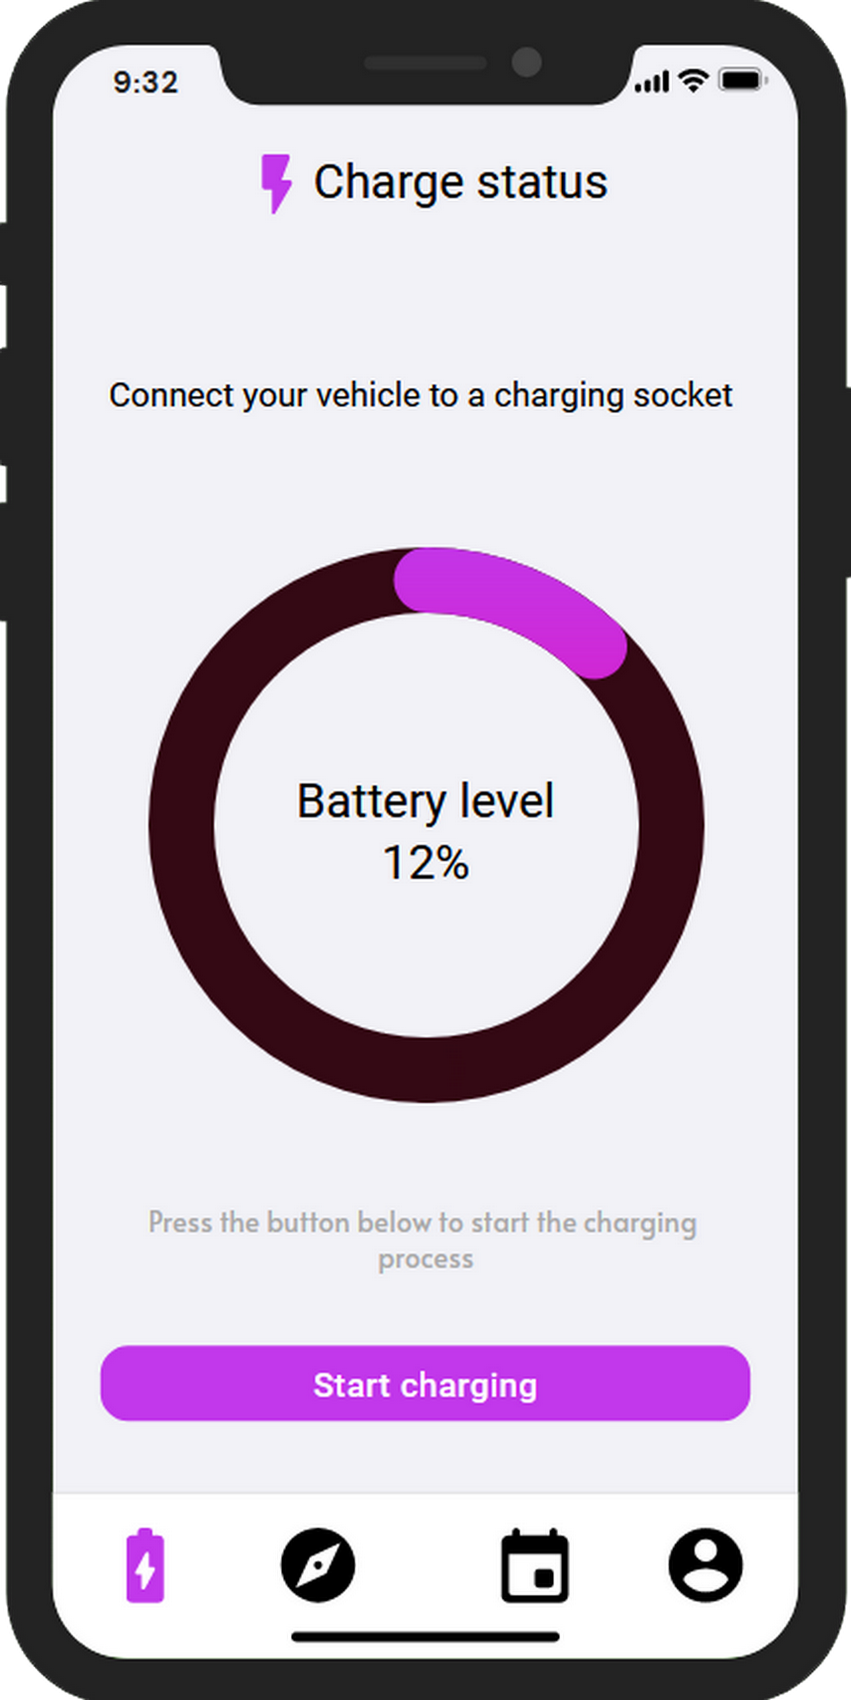
\includegraphics[width=30mm]{images/startcharge.png}\captionof{figure}{Charge status (start)}\label{fig:startProcess} &
  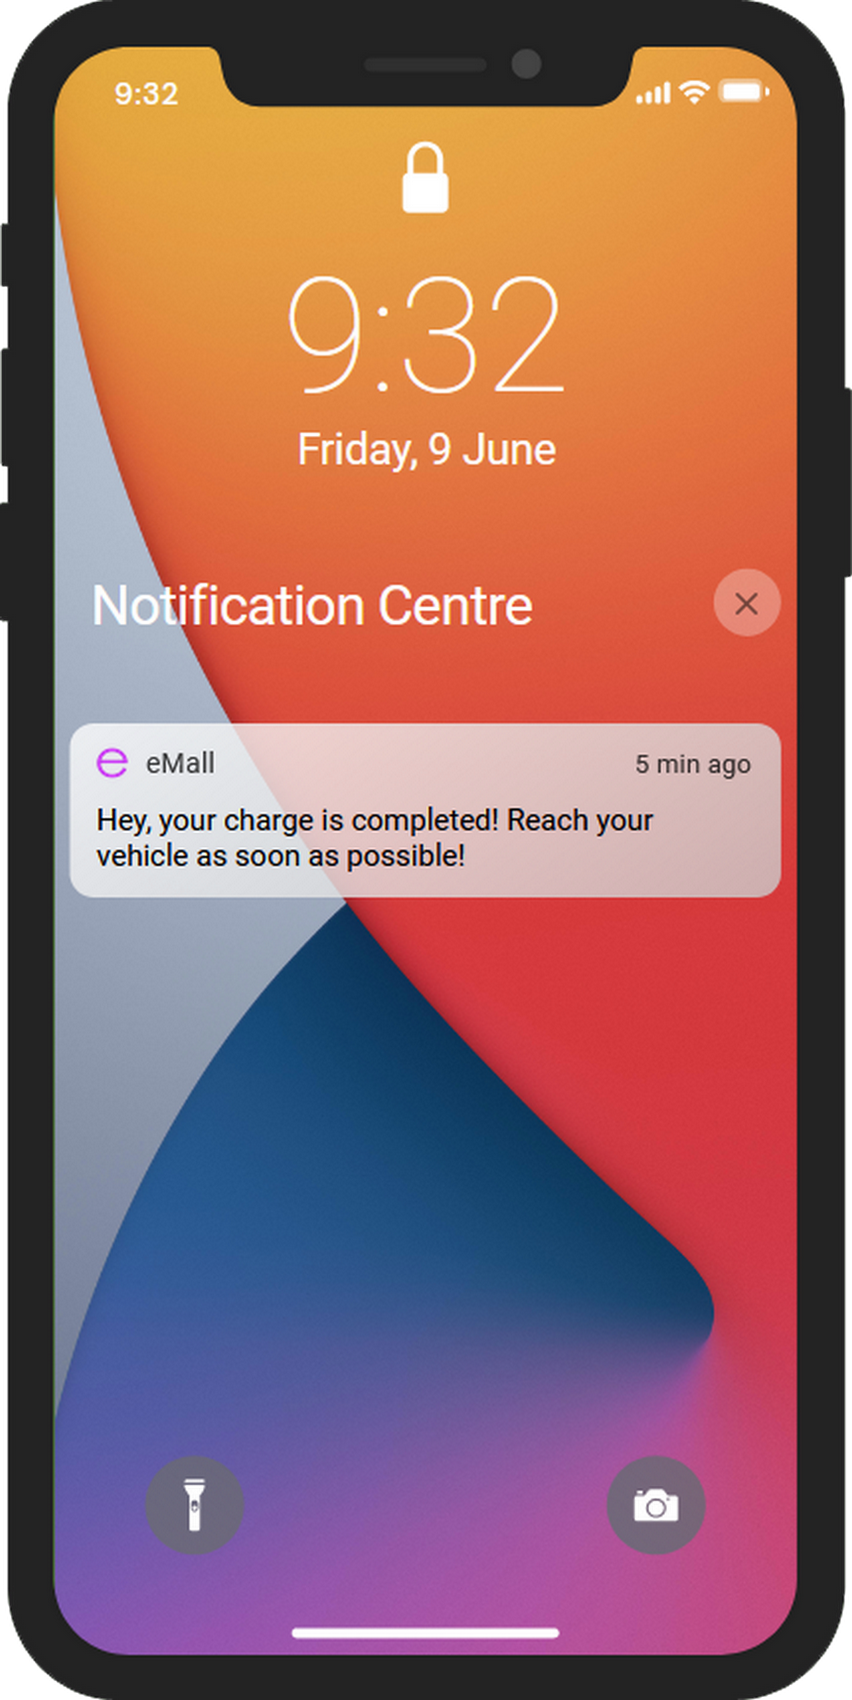
\includegraphics[width=30mm]{images/notific.png}\captionof{figure}{Notification}\label{fig:notificationView} \\
  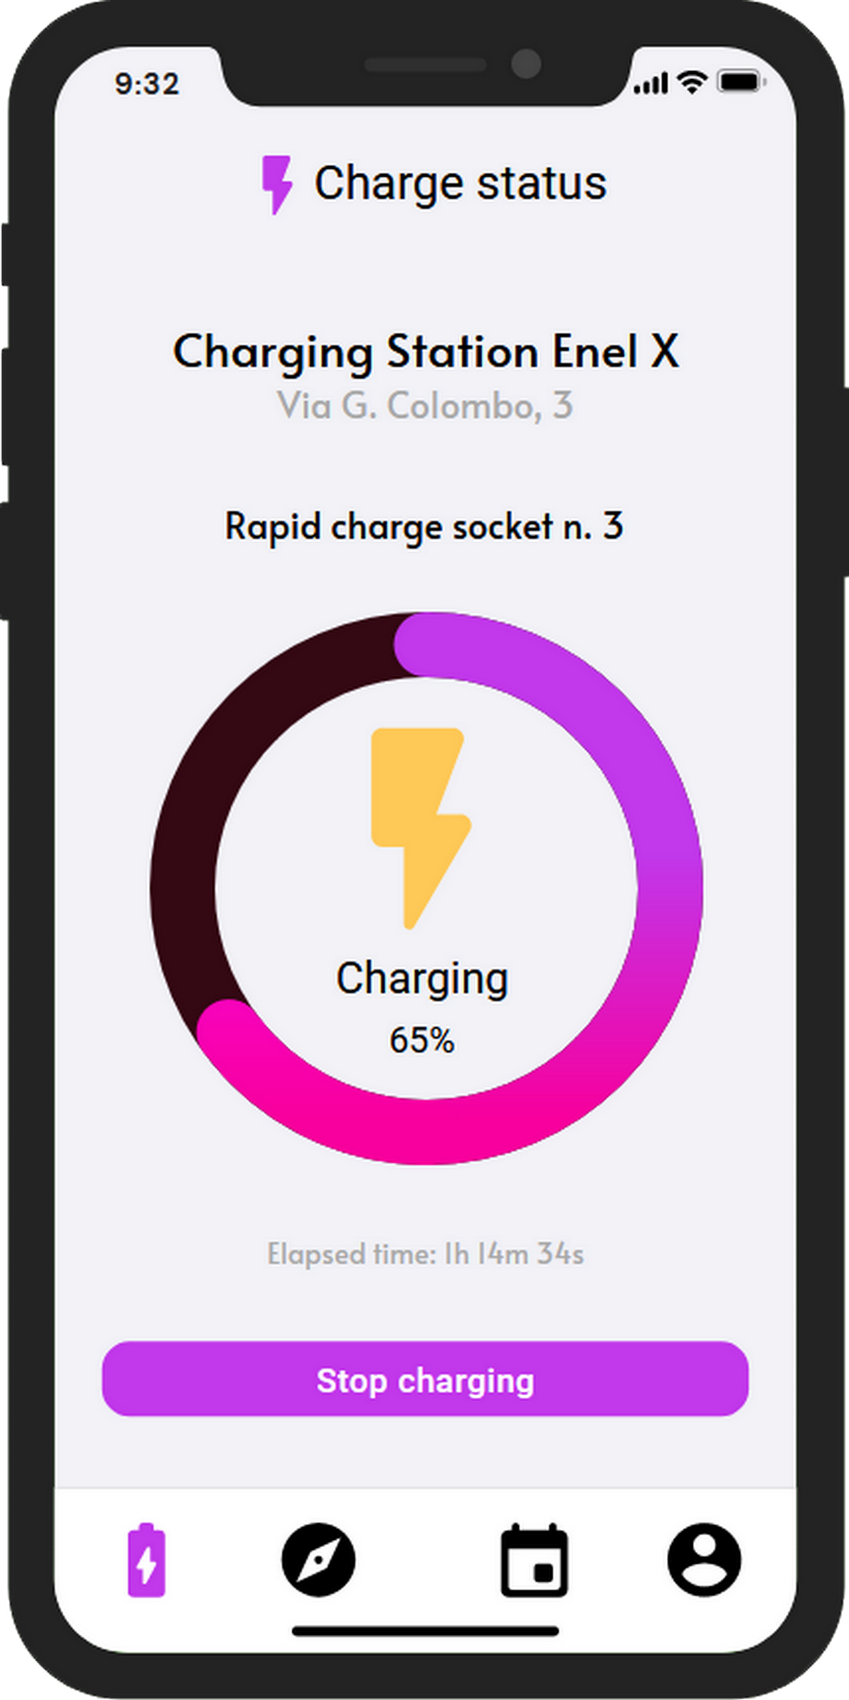
\includegraphics[width=30mm]{images/stopcharge.png}\captionof{figure}{Charge status (stop)}\label{fig:stopProcess} &
  
\includegraphics[width=30mm]{images/user.png}\captionof{figure}{Personal information}\label{fig:personalInformation} \\
\end{tabu}
\end{table}
The above mockups can be described as follows:
\begin{itemize}
    \item \textbf{Figure \ref{fig:homePageeMSP}}: The home page, allows the end user to choose between login and registration.
    \item \textbf{Figure \ref{fig:signUpPage}}: The sign up page, allows the end user to register himself.
    \item \textbf{Figure \ref{fig:logInPage}}: The log-in page, allows the end user to access the created profile and use the app.
    \item \textbf{Figure \ref{fig:chargingStationMap}}: The charging stations map, allows the end user to view the charging stations closest to him and to select the desired one.
    \item \textbf{Figure \ref{fig:bookingPage}}: The "My bookings page" allows the end user to view past, present and future bookings. It is also possible to view where the reservations were made and by clicking on it you can get more details.
    \item \textbf{Figure \ref{fig:qrCodePage}}: The "Booking details page", allows the end user to view more details of the reservation such as: time, date, name of the charging station, name of the street, type of socket and number. It is also possible to view the Qr-Code of the reservation, which must be shown to the scanner installed on the charging sockets to allow the supply of energy. If necessary, it is possible to cancel the reservation.
    \item \textbf{Figure \ref{fig:startProcess}}: The "Charge status page" allows the end user to view the status of his vehicle's battery and to start the charging process.
    \item \textbf{Figure \ref{fig:notificationView}}: The eMall application sends a notification to the end user when his vehicle recharging process is finished.
    \item \textbf{Figure \ref{fig:stopProcess}}: This is the same page of the \textbf{figure \ref{fig:startProcess}}, after starting the charging process, if necessary, it will be possible to stop it.
    \item \textbf{Figure \ref{fig:personalInformation}}: There is possible for the end user to view or modify their personal information such as: name, surname, email, password, credit cards. In addition, the end user can give consent to the use of GPS and own calendar.
\end{itemize}  
\newpage
The CPOs use a web based interface to take advantage of the features provided by the CPMS. The CPO admins can login at the same interface as well with credential. The mockpus of the interfaces are shown below.\\
\begin{table}[H]
\centering
\begin{tabu}to \textwidth {X[c]X[c]}
  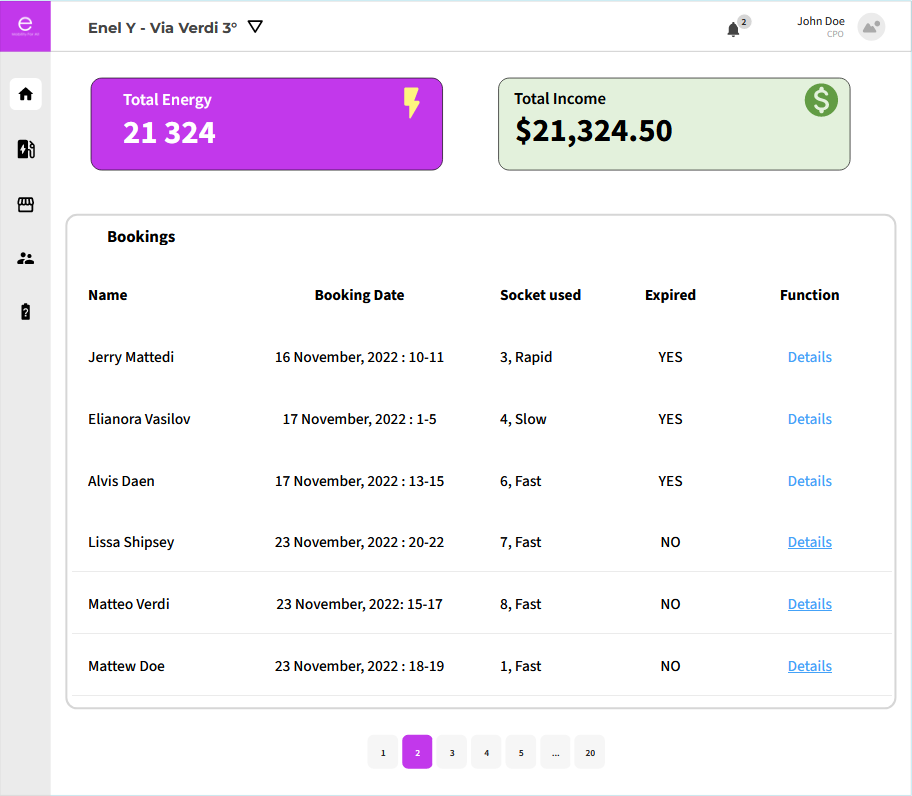
\includegraphics[width=70mm]{images/home2.png}\captionof{figure}{Home page}\label{fig:homePageCPO} &
  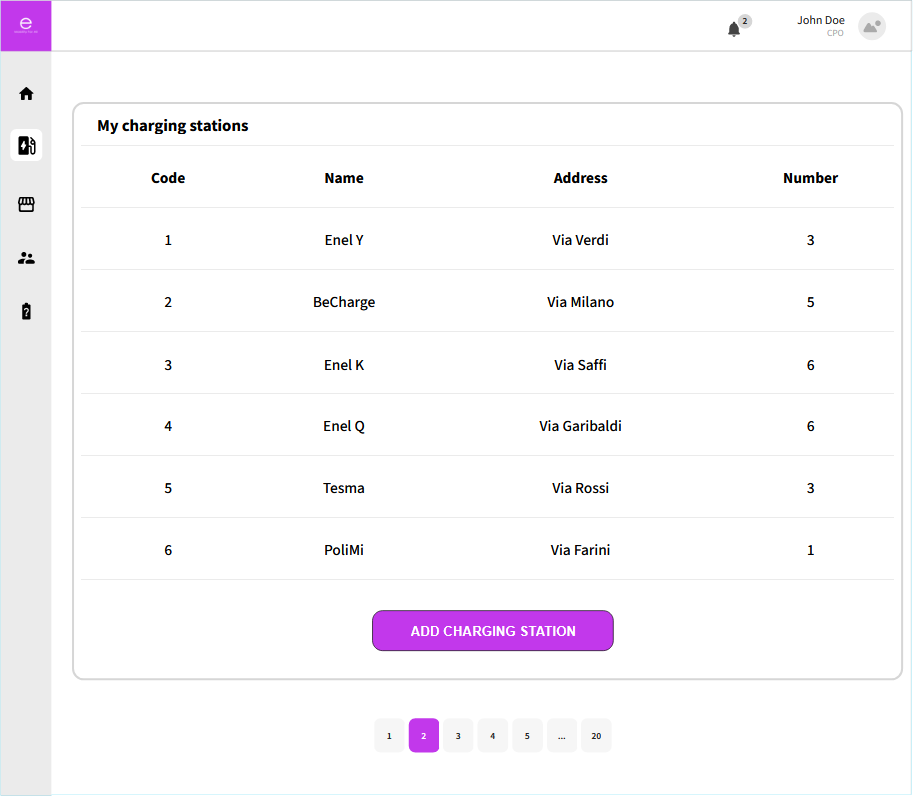
\includegraphics[width=70mm]{images/add.png}\captionof{figure}{My charging stations}\label{fig:chargingStation} \\
  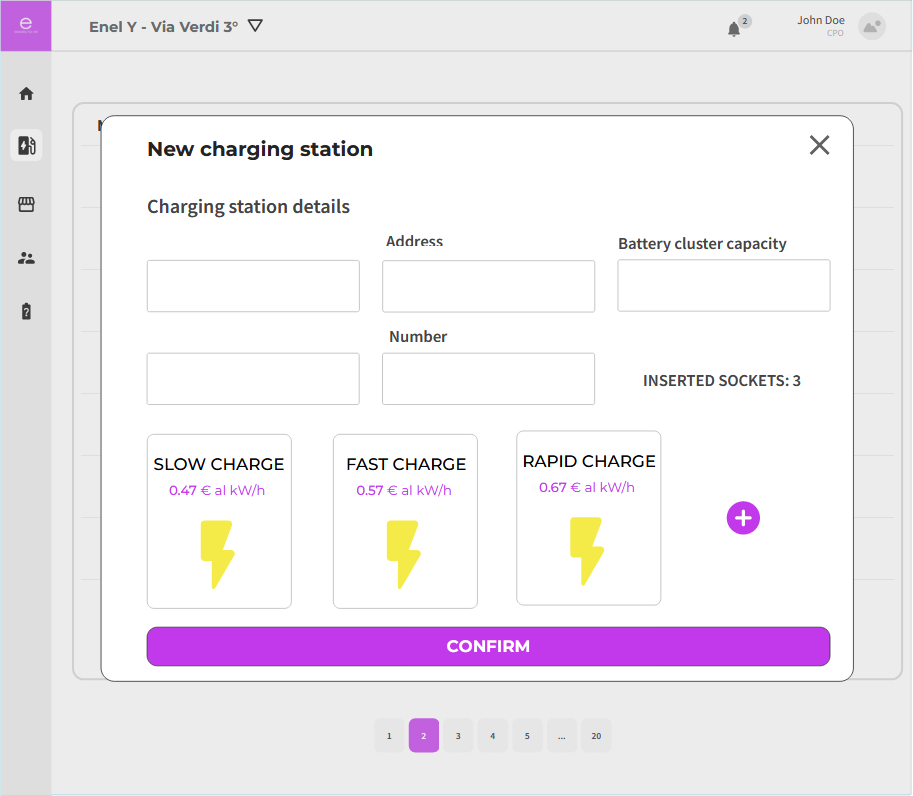
\includegraphics[width=70mm]{images/add2.png}\captionof{figure}{Add charging station}\label{fig:addChargingStation} &
  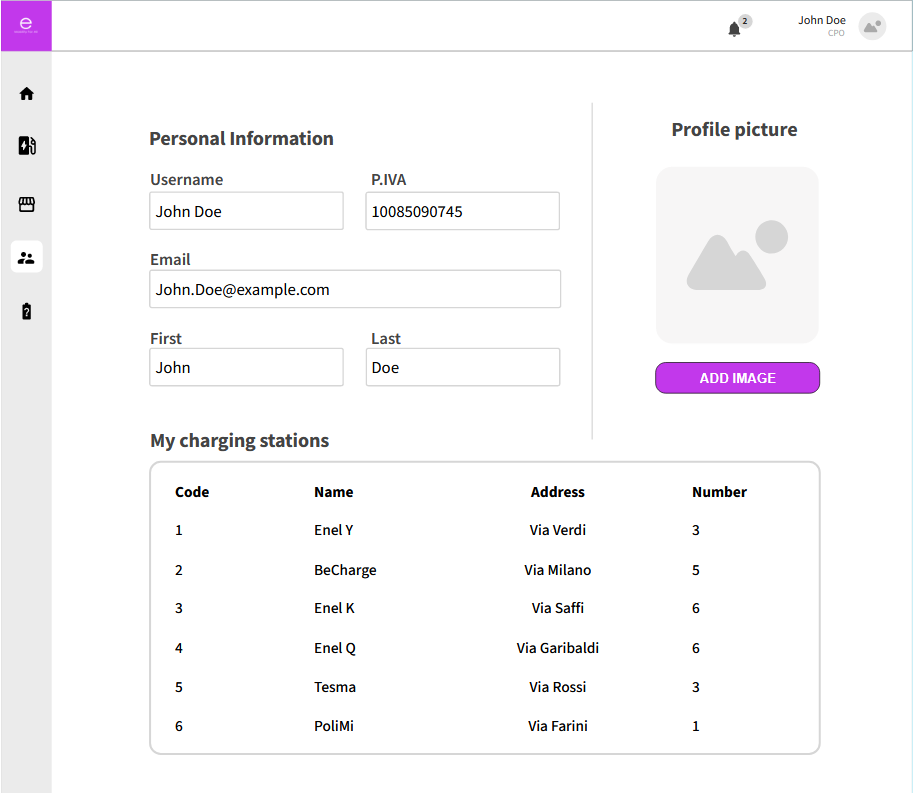
\includegraphics[width=70mm]{images/cpo.png}\captionof{figure}{Personal information}\label{fig:personalInformationCPO} \\
\end{tabu}
\end{table}
\begin{table}[H]
\centering
\begin{tabu}to \textwidth {X[c]X[c]}
  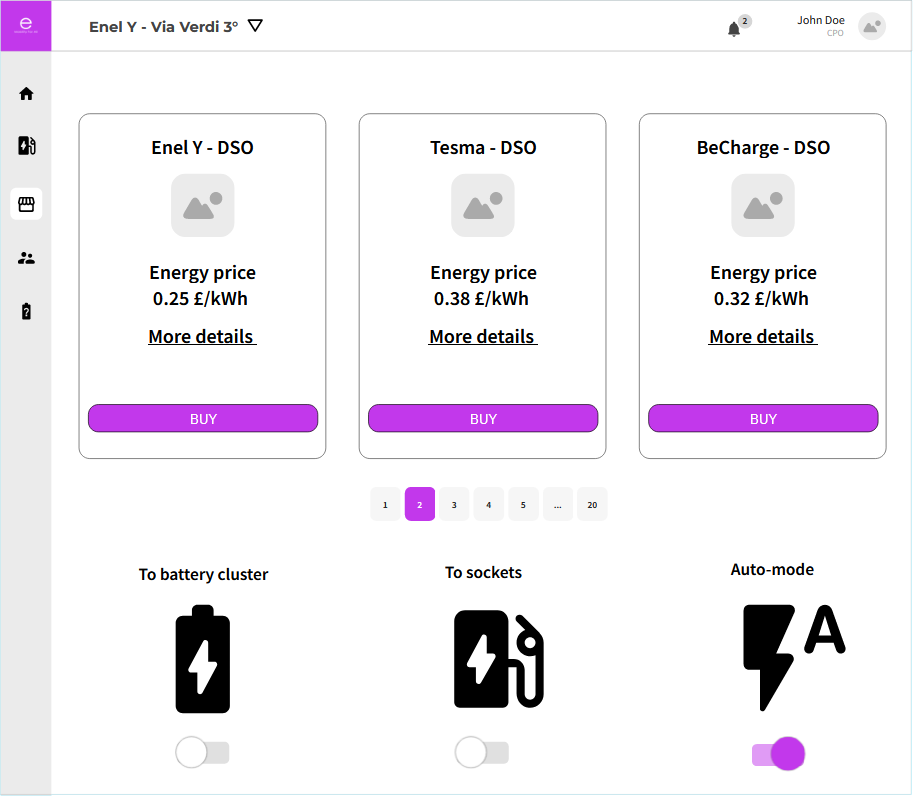
\includegraphics[width=70mm]{images/dso.png}\captionof{figure}{DSO interaction}\label{fig:dsoInteraction} &
  
\includegraphics[width=70mm]{images/battery.png}\captionof{figure}{Battery cluster status}\label{fig:batteryClusterStatus} \\\\
\end{tabu}
\end{table}
The above mockups can be described as follows:
\begin{itemize}
    \item \textbf{Figure \ref{fig:homePageCPO}}: The home page allows CPO to visualize reservations made in his charging stations.
    \item \textbf{Figure \ref{fig:chargingStation}}: There the CPO have a list of its charging stations with the related information: code, name, street. He can also add other charging station.
    \item \textbf{Figure \ref{fig:addChargingStation}}: By adding specific information required by the system, the CPO can add a new charging station with specific charging socket.
    \item \textbf{Figure \ref{fig:personalInformationCPO}}: There is possible for the CPO to view or modify their personal information such as: username, email, name, surname, password and company address.
    \item \textbf{Figure \ref{fig:dsoInteraction}}: It is possible, for the CPOs, to view various offers made by the DSOs for energy and to buy it from the offer they deem most valid. Furthermore, here he can decide on how to manage the energy he has just bought.
    \item \textbf{Figure \ref{fig:batteryClusterStatus}}: The "Battery cluster status page", allows the CPO to view more details of the Battery cluster such as: status, percentage, kW\_h TOT.,  kW\_h REMAINING, connected sockets. 
\end{itemize}  
\section{End User Interface Flow Diagram}
\begin{figure}[H]
    \centering
    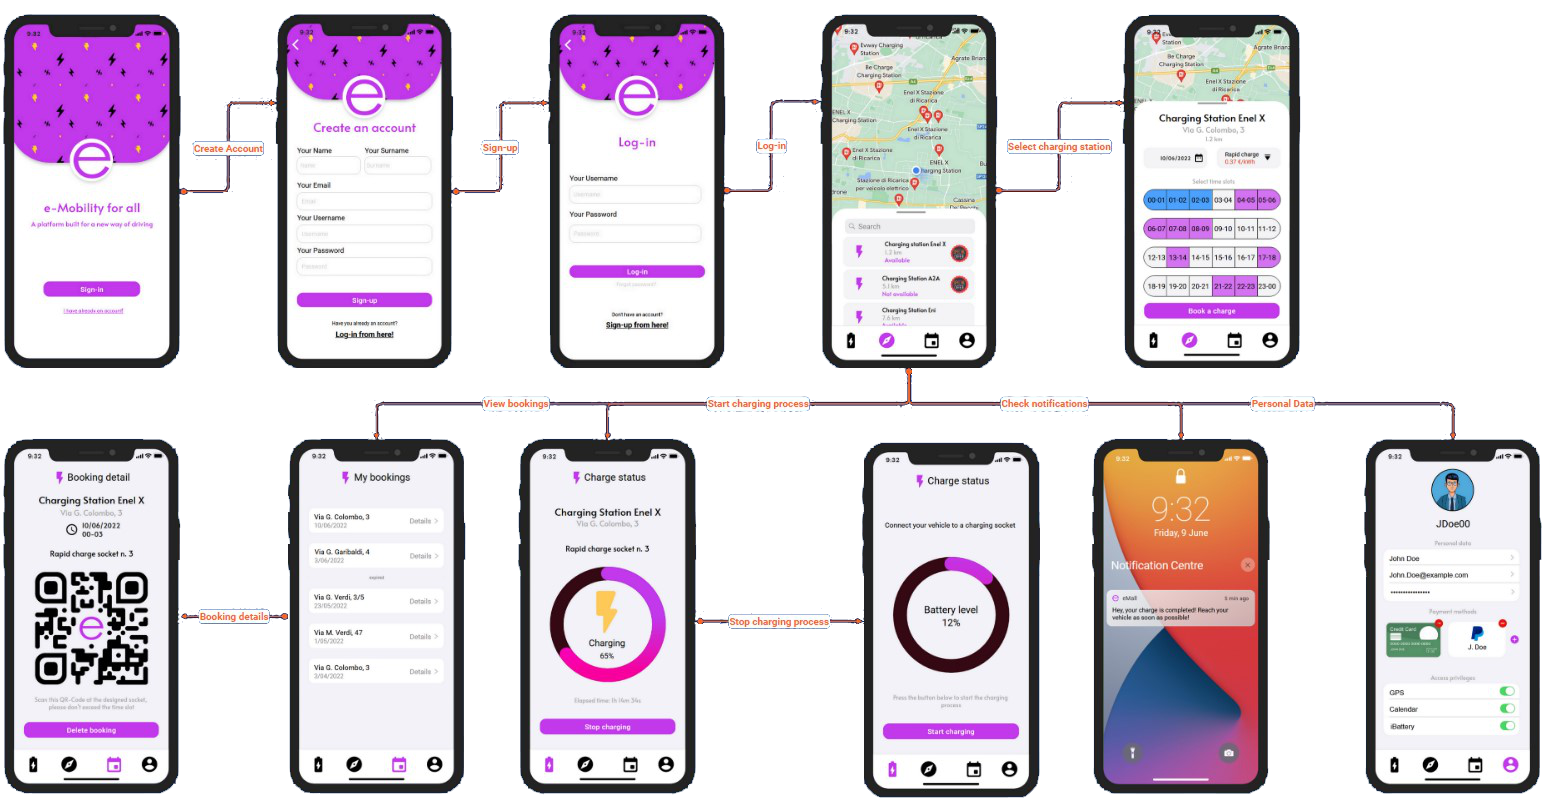
\includegraphics[width=\textwidth]{images/EndUserFlowDiagram.png}
    \caption{End User Interface Flow Diagram}
    \label{fig:EndUserFlowDiagram}
\end{figure}
\section{CPO Interface Flow Diagram}
\begin{figure}[H]
    \centering
    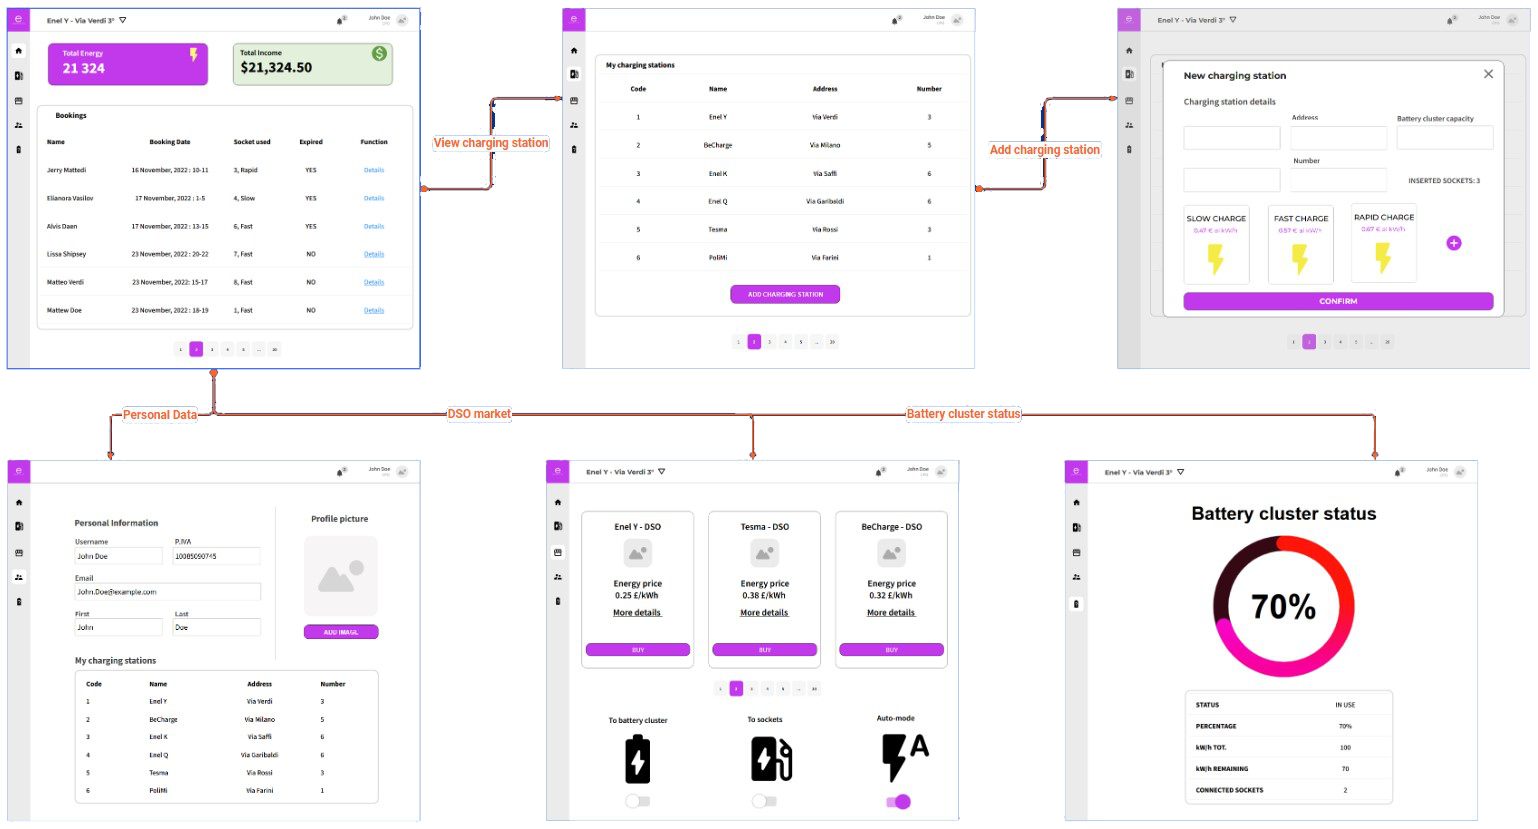
\includegraphics[width=\textwidth]{images/CPOflowDiagram.png}
    \caption{CPO Interface Flow Diagram}
    \label{fig:CPOFlowDiagram}
\end{figure}